% Created by tikzDevice version 0.11 on 2018-04-23 15:45:28
% !TEX encoding = UTF-8 Unicode
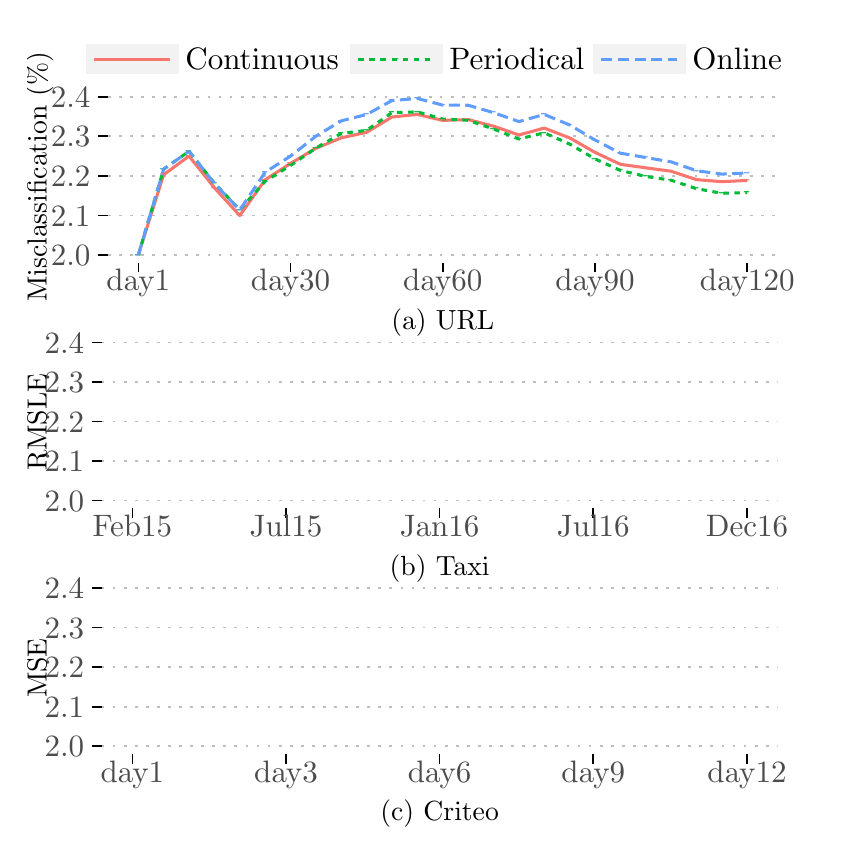
\begin{tikzpicture}[x=1pt,y=1pt]
\definecolor{fillColor}{RGB}{255,255,255}
\path[use as bounding box,fill=fillColor,fill opacity=0.00] (0,0) rectangle (289.08,289.08);
\begin{scope}
\path[clip] (  0.00,  0.00) rectangle (289.08,289.08);
\definecolor{fillColor}{RGB}{255,255,255}

\path[fill=fillColor] ( 10.68,266.32) rectangle (278.40,289.08);
\end{scope}
\begin{scope}
\path[clip] (  0.00,  0.00) rectangle (289.08,289.08);
\definecolor{drawColor}{RGB}{255,255,255}
\definecolor{fillColor}{gray}{0.95}

\path[draw=drawColor,line width= 0.6pt,line join=round,line cap=round,fill=fillColor] ( 20.71,272.01) rectangle ( 54.85,283.39);
\end{scope}
\begin{scope}
\path[clip] (  0.00,  0.00) rectangle (289.08,289.08);
\definecolor{drawColor}{RGB}{248,118,109}

\path[draw=drawColor,line width= 1.1pt,line join=round] ( 24.12,277.70) -- ( 51.43,277.70);
\end{scope}
\begin{scope}
\path[clip] (  0.00,  0.00) rectangle (289.08,289.08);
\definecolor{drawColor}{RGB}{248,118,109}

\node[text=drawColor,anchor=base,inner sep=0pt, outer sep=0pt, scale=  0.72] at ( 37.78,276.15) {-};
\end{scope}
\begin{scope}
\path[clip] (  0.00,  0.00) rectangle (289.08,289.08);
\definecolor{drawColor}{RGB}{255,255,255}
\definecolor{fillColor}{gray}{0.95}

\path[draw=drawColor,line width= 0.6pt,line join=round,line cap=round,fill=fillColor] (116.06,272.01) rectangle (150.20,283.39);
\end{scope}
\begin{scope}
\path[clip] (  0.00,  0.00) rectangle (289.08,289.08);
\definecolor{drawColor}{RGB}{0,186,56}

\path[draw=drawColor,line width= 1.1pt,dash pattern=on 2pt off 2pt ,line join=round] (119.47,277.70) -- (146.79,277.70);
\end{scope}
\begin{scope}
\path[clip] (  0.00,  0.00) rectangle (289.08,289.08);
\definecolor{drawColor}{RGB}{0,186,56}

\node[text=drawColor,anchor=base,inner sep=0pt, outer sep=0pt, scale=  0.72] at (133.13,276.15) {-};
\end{scope}
\begin{scope}
\path[clip] (  0.00,  0.00) rectangle (289.08,289.08);
\definecolor{drawColor}{RGB}{255,255,255}
\definecolor{fillColor}{gray}{0.95}

\path[draw=drawColor,line width= 0.6pt,line join=round,line cap=round,fill=fillColor] (203.90,272.01) rectangle (238.05,283.39);
\end{scope}
\begin{scope}
\path[clip] (  0.00,  0.00) rectangle (289.08,289.08);
\definecolor{drawColor}{RGB}{97,156,255}

\path[draw=drawColor,line width= 1.1pt,dash pattern=on 4pt off 2pt ,line join=round] (207.32,277.70) -- (234.63,277.70);
\end{scope}
\begin{scope}
\path[clip] (  0.00,  0.00) rectangle (289.08,289.08);
\definecolor{drawColor}{RGB}{97,156,255}

\node[text=drawColor,anchor=base,inner sep=0pt, outer sep=0pt, scale=  0.72] at (220.97,276.15) {-};
\end{scope}
\begin{scope}
\path[clip] (  0.00,  0.00) rectangle (289.08,289.08);
\definecolor{drawColor}{RGB}{0,0,0}

\node[text=drawColor,anchor=base west,inner sep=0pt, outer sep=0pt, scale=  1.12] at ( 57.02,273.84) {Continuous};
\end{scope}
\begin{scope}
\path[clip] (  0.00,  0.00) rectangle (289.08,289.08);
\definecolor{drawColor}{RGB}{0,0,0}

\node[text=drawColor,anchor=base west,inner sep=0pt, outer sep=0pt, scale=  1.12] at (152.37,273.84) {Periodical};
\end{scope}
\begin{scope}
\path[clip] (  0.00,  0.00) rectangle (289.08,289.08);
\definecolor{drawColor}{RGB}{0,0,0}

\node[text=drawColor,anchor=base west,inner sep=0pt, outer sep=0pt, scale=  1.12] at (240.21,273.84) {Online};
\end{scope}
\begin{scope}
\path[clip] (  0.00,177.55) rectangle (289.08,266.32);
\definecolor{drawColor}{RGB}{255,255,255}
\definecolor{fillColor}{RGB}{255,255,255}

\path[draw=drawColor,line width= 0.6pt,line join=round,line cap=round,fill=fillColor] (  0.00,177.55) rectangle (289.08,266.32);
\end{scope}
\begin{scope}
\path[clip] ( 28.99,204.14) rectangle (271.01,266.32);
\definecolor{fillColor}{RGB}{255,255,255}

\path[fill=fillColor] ( 28.99,204.14) rectangle (271.01,266.32);
\definecolor{drawColor}{RGB}{255,255,255}

\path[draw=drawColor,line width= 0.3pt,line join=round] ( 28.99,214.11) --
	(271.01,214.11);

\path[draw=drawColor,line width= 0.3pt,line join=round] ( 28.99,228.40) --
	(271.01,228.40);

\path[draw=drawColor,line width= 0.3pt,line join=round] ( 28.99,242.68) --
	(271.01,242.68);

\path[draw=drawColor,line width= 0.3pt,line join=round] ( 28.99,256.97) --
	(271.01,256.97);

\path[draw=drawColor,line width= 0.3pt,line join=round] ( 67.49,204.14) --
	( 67.49,266.32);

\path[draw=drawColor,line width= 0.3pt,line join=round] (122.49,204.14) --
	(122.49,266.32);

\path[draw=drawColor,line width= 0.3pt,line join=round] (177.50,204.14) --
	(177.50,266.32);

\path[draw=drawColor,line width= 0.3pt,line join=round] (232.51,204.14) --
	(232.51,266.32);
\definecolor{drawColor}{RGB}{190,190,190}

\path[draw=drawColor,line width= 0.6pt,dash pattern=on 1pt off 3pt ,line join=round] ( 28.99,206.97) --
	(271.01,206.97);

\path[draw=drawColor,line width= 0.6pt,dash pattern=on 1pt off 3pt ,line join=round] ( 28.99,221.25) --
	(271.01,221.25);

\path[draw=drawColor,line width= 0.6pt,dash pattern=on 1pt off 3pt ,line join=round] ( 28.99,235.54) --
	(271.01,235.54);

\path[draw=drawColor,line width= 0.6pt,dash pattern=on 1pt off 3pt ,line join=round] ( 28.99,249.83) --
	(271.01,249.83);

\path[draw=drawColor,line width= 0.6pt,dash pattern=on 1pt off 3pt ,line join=round] ( 28.99,264.11) --
	(271.01,264.11);
\definecolor{drawColor}{RGB}{255,255,255}

\path[draw=drawColor,line width= 0.6pt,line join=round] ( 39.99,204.14) --
	( 39.99,266.32);

\path[draw=drawColor,line width= 0.6pt,line join=round] ( 94.98,204.14) --
	( 94.98,266.32);

\path[draw=drawColor,line width= 0.6pt,line join=round] (149.99,204.14) --
	(149.99,266.32);

\path[draw=drawColor,line width= 0.6pt,line join=round] (205.00,204.14) --
	(205.00,266.32);

\path[draw=drawColor,line width= 0.6pt,line join=round] (260.01,204.14) --
	(260.01,266.32);
\definecolor{drawColor}{RGB}{248,118,109}

\path[draw=drawColor,line width= 1.1pt,line join=round] ( 39.99,206.97) --
	( 49.14,235.97) --
	( 58.31,242.68) --
	( 67.48,231.21) --
	( 76.64,221.18) --
	( 85.81,234.11) --
	( 94.98,240.02) --
	(104.15,245.48) --
	(113.32,249.26) --
	(122.49,251.27) --
	(131.65,256.80) --
	(140.82,257.72) --
	(149.99,255.57) --
	(159.16,255.87) --
	(168.33,253.49) --
	(177.50,250.30) --
	(186.66,252.79) --
	(195.83,249.25) --
	(205.00,244.02) --
	(214.17,239.70) --
	(223.34,238.43) --
	(232.51,237.20) --
	(241.67,234.16) --
	(250.84,233.43) --
	(260.01,233.87);
\definecolor{drawColor}{RGB}{0,186,56}

\path[draw=drawColor,line width= 1.1pt,dash pattern=on 2pt off 2pt ,line join=round] ( 39.99,206.97) --
	( 49.14,237.97) --
	( 58.31,244.40) --
	( 67.48,232.87) --
	( 76.64,223.29) --
	( 85.81,233.57) --
	( 94.98,239.28) --
	(104.15,245.58) --
	(113.32,250.86) --
	(122.49,251.97) --
	(131.65,258.38) --
	(140.82,258.64) --
	(149.99,256.06) --
	(159.16,255.62) --
	(168.33,252.46) --
	(177.50,248.84) --
	(186.66,251.08) --
	(195.83,247.02) --
	(205.00,241.66) --
	(214.17,237.49) --
	(223.34,235.35) --
	(232.51,233.94) --
	(241.67,230.91) --
	(250.84,229.23) --
	(260.01,229.47);
\definecolor{drawColor}{RGB}{97,156,255}

\path[draw=drawColor,line width= 1.1pt,dash pattern=on 4pt off 2pt ,line join=round] ( 39.99,206.97) --
	( 49.14,237.97) --
	( 58.31,244.40) --
	( 67.48,232.78) --
	( 76.64,223.22) --
	( 85.81,236.83) --
	( 94.98,242.66) --
	(104.15,249.85) --
	(113.32,255.42) --
	(122.49,257.70) --
	(131.65,262.74) --
	(140.82,263.49) --
	(149.99,261.10) --
	(159.16,261.04) --
	(168.33,258.38) --
	(177.50,255.14) --
	(186.66,257.72) --
	(195.83,253.93) --
	(205.00,248.50) --
	(214.17,243.72) --
	(223.34,242.16) --
	(232.51,240.58) --
	(241.67,237.38) --
	(250.84,236.16) --
	(260.01,236.57);
\definecolor{drawColor}{RGB}{248,118,109}

\node[text=drawColor,anchor=base,inner sep=0pt, outer sep=0pt, scale=  0.72] at ( 39.99,205.42) {-};

\node[text=drawColor,anchor=base,inner sep=0pt, outer sep=0pt, scale=  0.72] at ( 49.14,234.42) {-};

\node[text=drawColor,anchor=base,inner sep=0pt, outer sep=0pt, scale=  0.72] at ( 58.31,241.13) {-};

\node[text=drawColor,anchor=base,inner sep=0pt, outer sep=0pt, scale=  0.72] at ( 67.48,229.66) {-};

\node[text=drawColor,anchor=base,inner sep=0pt, outer sep=0pt, scale=  0.72] at ( 76.64,219.63) {-};

\node[text=drawColor,anchor=base,inner sep=0pt, outer sep=0pt, scale=  0.72] at ( 85.81,232.56) {-};

\node[text=drawColor,anchor=base,inner sep=0pt, outer sep=0pt, scale=  0.72] at ( 94.98,238.47) {-};

\node[text=drawColor,anchor=base,inner sep=0pt, outer sep=0pt, scale=  0.72] at (104.15,243.93) {-};

\node[text=drawColor,anchor=base,inner sep=0pt, outer sep=0pt, scale=  0.72] at (113.32,247.71) {-};

\node[text=drawColor,anchor=base,inner sep=0pt, outer sep=0pt, scale=  0.72] at (122.49,249.72) {-};

\node[text=drawColor,anchor=base,inner sep=0pt, outer sep=0pt, scale=  0.72] at (131.65,255.24) {-};

\node[text=drawColor,anchor=base,inner sep=0pt, outer sep=0pt, scale=  0.72] at (140.82,256.17) {-};

\node[text=drawColor,anchor=base,inner sep=0pt, outer sep=0pt, scale=  0.72] at (149.99,254.02) {-};

\node[text=drawColor,anchor=base,inner sep=0pt, outer sep=0pt, scale=  0.72] at (159.16,254.32) {-};

\node[text=drawColor,anchor=base,inner sep=0pt, outer sep=0pt, scale=  0.72] at (168.33,251.94) {-};

\node[text=drawColor,anchor=base,inner sep=0pt, outer sep=0pt, scale=  0.72] at (177.50,248.75) {-};

\node[text=drawColor,anchor=base,inner sep=0pt, outer sep=0pt, scale=  0.72] at (186.66,251.24) {-};

\node[text=drawColor,anchor=base,inner sep=0pt, outer sep=0pt, scale=  0.72] at (195.83,247.70) {-};

\node[text=drawColor,anchor=base,inner sep=0pt, outer sep=0pt, scale=  0.72] at (205.00,242.47) {-};

\node[text=drawColor,anchor=base,inner sep=0pt, outer sep=0pt, scale=  0.72] at (214.17,238.15) {-};

\node[text=drawColor,anchor=base,inner sep=0pt, outer sep=0pt, scale=  0.72] at (223.34,236.88) {-};

\node[text=drawColor,anchor=base,inner sep=0pt, outer sep=0pt, scale=  0.72] at (232.51,235.65) {-};

\node[text=drawColor,anchor=base,inner sep=0pt, outer sep=0pt, scale=  0.72] at (241.67,232.61) {-};

\node[text=drawColor,anchor=base,inner sep=0pt, outer sep=0pt, scale=  0.72] at (250.84,231.88) {-};

\node[text=drawColor,anchor=base,inner sep=0pt, outer sep=0pt, scale=  0.72] at (260.01,232.32) {-};
\definecolor{drawColor}{RGB}{0,186,56}

\node[text=drawColor,anchor=base,inner sep=0pt, outer sep=0pt, scale=  0.72] at ( 39.99,205.42) {-};

\node[text=drawColor,anchor=base,inner sep=0pt, outer sep=0pt, scale=  0.72] at ( 49.14,236.42) {-};

\node[text=drawColor,anchor=base,inner sep=0pt, outer sep=0pt, scale=  0.72] at ( 58.31,242.85) {-};

\node[text=drawColor,anchor=base,inner sep=0pt, outer sep=0pt, scale=  0.72] at ( 67.48,231.32) {-};

\node[text=drawColor,anchor=base,inner sep=0pt, outer sep=0pt, scale=  0.72] at ( 76.64,221.74) {-};

\node[text=drawColor,anchor=base,inner sep=0pt, outer sep=0pt, scale=  0.72] at ( 85.81,232.02) {-};

\node[text=drawColor,anchor=base,inner sep=0pt, outer sep=0pt, scale=  0.72] at ( 94.98,237.73) {-};

\node[text=drawColor,anchor=base,inner sep=0pt, outer sep=0pt, scale=  0.72] at (104.15,244.03) {-};

\node[text=drawColor,anchor=base,inner sep=0pt, outer sep=0pt, scale=  0.72] at (113.32,249.31) {-};

\node[text=drawColor,anchor=base,inner sep=0pt, outer sep=0pt, scale=  0.72] at (122.49,250.42) {-};

\node[text=drawColor,anchor=base,inner sep=0pt, outer sep=0pt, scale=  0.72] at (131.65,256.83) {-};

\node[text=drawColor,anchor=base,inner sep=0pt, outer sep=0pt, scale=  0.72] at (140.82,257.09) {-};

\node[text=drawColor,anchor=base,inner sep=0pt, outer sep=0pt, scale=  0.72] at (149.99,254.51) {-};

\node[text=drawColor,anchor=base,inner sep=0pt, outer sep=0pt, scale=  0.72] at (159.16,254.07) {-};

\node[text=drawColor,anchor=base,inner sep=0pt, outer sep=0pt, scale=  0.72] at (168.33,250.91) {-};

\node[text=drawColor,anchor=base,inner sep=0pt, outer sep=0pt, scale=  0.72] at (177.50,247.29) {-};

\node[text=drawColor,anchor=base,inner sep=0pt, outer sep=0pt, scale=  0.72] at (186.66,249.52) {-};

\node[text=drawColor,anchor=base,inner sep=0pt, outer sep=0pt, scale=  0.72] at (195.83,245.47) {-};

\node[text=drawColor,anchor=base,inner sep=0pt, outer sep=0pt, scale=  0.72] at (205.00,240.11) {-};

\node[text=drawColor,anchor=base,inner sep=0pt, outer sep=0pt, scale=  0.72] at (214.17,235.94) {-};

\node[text=drawColor,anchor=base,inner sep=0pt, outer sep=0pt, scale=  0.72] at (223.34,233.80) {-};

\node[text=drawColor,anchor=base,inner sep=0pt, outer sep=0pt, scale=  0.72] at (232.51,232.39) {-};

\node[text=drawColor,anchor=base,inner sep=0pt, outer sep=0pt, scale=  0.72] at (241.67,229.36) {-};

\node[text=drawColor,anchor=base,inner sep=0pt, outer sep=0pt, scale=  0.72] at (250.84,227.68) {-};

\node[text=drawColor,anchor=base,inner sep=0pt, outer sep=0pt, scale=  0.72] at (260.01,227.92) {-};
\definecolor{drawColor}{RGB}{97,156,255}

\node[text=drawColor,anchor=base,inner sep=0pt, outer sep=0pt, scale=  0.72] at ( 39.99,205.42) {-};

\node[text=drawColor,anchor=base,inner sep=0pt, outer sep=0pt, scale=  0.72] at ( 49.14,236.42) {-};

\node[text=drawColor,anchor=base,inner sep=0pt, outer sep=0pt, scale=  0.72] at ( 58.31,242.85) {-};

\node[text=drawColor,anchor=base,inner sep=0pt, outer sep=0pt, scale=  0.72] at ( 67.48,231.23) {-};

\node[text=drawColor,anchor=base,inner sep=0pt, outer sep=0pt, scale=  0.72] at ( 76.64,221.67) {-};

\node[text=drawColor,anchor=base,inner sep=0pt, outer sep=0pt, scale=  0.72] at ( 85.81,235.28) {-};

\node[text=drawColor,anchor=base,inner sep=0pt, outer sep=0pt, scale=  0.72] at ( 94.98,241.11) {-};

\node[text=drawColor,anchor=base,inner sep=0pt, outer sep=0pt, scale=  0.72] at (104.15,248.30) {-};

\node[text=drawColor,anchor=base,inner sep=0pt, outer sep=0pt, scale=  0.72] at (113.32,253.87) {-};

\node[text=drawColor,anchor=base,inner sep=0pt, outer sep=0pt, scale=  0.72] at (122.49,256.15) {-};

\node[text=drawColor,anchor=base,inner sep=0pt, outer sep=0pt, scale=  0.72] at (131.65,261.19) {-};

\node[text=drawColor,anchor=base,inner sep=0pt, outer sep=0pt, scale=  0.72] at (140.82,261.94) {-};

\node[text=drawColor,anchor=base,inner sep=0pt, outer sep=0pt, scale=  0.72] at (149.99,259.55) {-};

\node[text=drawColor,anchor=base,inner sep=0pt, outer sep=0pt, scale=  0.72] at (159.16,259.49) {-};

\node[text=drawColor,anchor=base,inner sep=0pt, outer sep=0pt, scale=  0.72] at (168.33,256.83) {-};

\node[text=drawColor,anchor=base,inner sep=0pt, outer sep=0pt, scale=  0.72] at (177.50,253.59) {-};

\node[text=drawColor,anchor=base,inner sep=0pt, outer sep=0pt, scale=  0.72] at (186.66,256.17) {-};

\node[text=drawColor,anchor=base,inner sep=0pt, outer sep=0pt, scale=  0.72] at (195.83,252.38) {-};

\node[text=drawColor,anchor=base,inner sep=0pt, outer sep=0pt, scale=  0.72] at (205.00,246.94) {-};

\node[text=drawColor,anchor=base,inner sep=0pt, outer sep=0pt, scale=  0.72] at (214.17,242.17) {-};

\node[text=drawColor,anchor=base,inner sep=0pt, outer sep=0pt, scale=  0.72] at (223.34,240.61) {-};

\node[text=drawColor,anchor=base,inner sep=0pt, outer sep=0pt, scale=  0.72] at (232.51,239.03) {-};

\node[text=drawColor,anchor=base,inner sep=0pt, outer sep=0pt, scale=  0.72] at (241.67,235.83) {-};

\node[text=drawColor,anchor=base,inner sep=0pt, outer sep=0pt, scale=  0.72] at (250.84,234.60) {-};

\node[text=drawColor,anchor=base,inner sep=0pt, outer sep=0pt, scale=  0.72] at (260.01,235.02) {-};
\end{scope}
\begin{scope}
\path[clip] (  0.00,  0.00) rectangle (289.08,289.08);
\definecolor{drawColor}{gray}{0.30}

\node[text=drawColor,anchor=base east,inner sep=0pt, outer sep=0pt, scale=  1.12] at ( 22.69,203.11) {2.0};

\node[text=drawColor,anchor=base east,inner sep=0pt, outer sep=0pt, scale=  1.12] at ( 22.69,217.40) {2.1};

\node[text=drawColor,anchor=base east,inner sep=0pt, outer sep=0pt, scale=  1.12] at ( 22.69,231.68) {2.2};

\node[text=drawColor,anchor=base east,inner sep=0pt, outer sep=0pt, scale=  1.12] at ( 22.69,245.97) {2.3};

\node[text=drawColor,anchor=base east,inner sep=0pt, outer sep=0pt, scale=  1.12] at ( 22.69,260.26) {2.4};
\end{scope}
\begin{scope}
\path[clip] (  0.00,  0.00) rectangle (289.08,289.08);
\definecolor{drawColor}{RGB}{0,0,0}

\path[draw=drawColor,line width= 0.6pt,line join=round] ( 25.49,206.97) --
	( 28.99,206.97);

\path[draw=drawColor,line width= 0.6pt,line join=round] ( 25.49,221.25) --
	( 28.99,221.25);

\path[draw=drawColor,line width= 0.6pt,line join=round] ( 25.49,235.54) --
	( 28.99,235.54);

\path[draw=drawColor,line width= 0.6pt,line join=round] ( 25.49,249.83) --
	( 28.99,249.83);

\path[draw=drawColor,line width= 0.6pt,line join=round] ( 25.49,264.11) --
	( 28.99,264.11);
\end{scope}
\begin{scope}
\path[clip] (  0.00,  0.00) rectangle (289.08,289.08);
\definecolor{drawColor}{RGB}{0,0,0}

\path[draw=drawColor,line width= 0.6pt,line join=round] ( 39.99,200.64) --
	( 39.99,204.14);

\path[draw=drawColor,line width= 0.6pt,line join=round] ( 94.98,200.64) --
	( 94.98,204.14);

\path[draw=drawColor,line width= 0.6pt,line join=round] (149.99,200.64) --
	(149.99,204.14);

\path[draw=drawColor,line width= 0.6pt,line join=round] (205.00,200.64) --
	(205.00,204.14);

\path[draw=drawColor,line width= 0.6pt,line join=round] (260.01,200.64) --
	(260.01,204.14);
\end{scope}
\begin{scope}
\path[clip] (  0.00,  0.00) rectangle (289.08,289.08);
\definecolor{drawColor}{gray}{0.30}

\node[text=drawColor,anchor=base,inner sep=0pt, outer sep=0pt, scale=  1.12] at ( 39.99,193.93) {day1};

\node[text=drawColor,anchor=base,inner sep=0pt, outer sep=0pt, scale=  1.12] at ( 94.98,193.93) {day30};

\node[text=drawColor,anchor=base,inner sep=0pt, outer sep=0pt, scale=  1.12] at (149.99,193.93) {day60};

\node[text=drawColor,anchor=base,inner sep=0pt, outer sep=0pt, scale=  1.12] at (205.00,193.93) {day90};

\node[text=drawColor,anchor=base,inner sep=0pt, outer sep=0pt, scale=  1.12] at (260.01,193.93) {day120};
\end{scope}
\begin{scope}
\path[clip] (  0.00,  0.00) rectangle (289.08,289.08);
\definecolor{drawColor}{RGB}{0,0,0}

\node[text=drawColor,anchor=base,inner sep=0pt, outer sep=0pt, scale=  1.00] at (150.00,180.04) {(a) URL};
\end{scope}
\begin{scope}
\path[clip] (  0.00,  0.00) rectangle (289.08,289.08);
\definecolor{drawColor}{RGB}{0,0,0}

\node[text=drawColor,rotate= 90.00,anchor=base,inner sep=0pt, outer sep=0pt, scale=  1.00] at (  6.89,235.23) {Misclassification (\%)};
\end{scope}
\begin{scope}
\path[clip] (  0.00, 88.77) rectangle (289.08,177.55);
\definecolor{drawColor}{RGB}{255,255,255}
\definecolor{fillColor}{RGB}{255,255,255}

\path[draw=drawColor,line width= 0.6pt,line join=round,line cap=round,fill=fillColor] (  0.00, 88.77) rectangle (289.08,177.55);
\end{scope}
\begin{scope}
\path[clip] ( 26.72,115.37) rectangle (271.01,177.55);
\definecolor{fillColor}{RGB}{255,255,255}

\path[fill=fillColor] ( 26.72,115.37) rectangle (271.01,177.55);
\definecolor{drawColor}{RGB}{255,255,255}

\path[draw=drawColor,line width= 0.3pt,line join=round] ( 26.72,125.34) --
	(271.01,125.34);

\path[draw=drawColor,line width= 0.3pt,line join=round] ( 26.72,139.62) --
	(271.01,139.62);

\path[draw=drawColor,line width= 0.3pt,line join=round] ( 26.72,153.91) --
	(271.01,153.91);

\path[draw=drawColor,line width= 0.3pt,line join=round] ( 26.72,168.20) --
	(271.01,168.20);

\path[draw=drawColor,line width= 0.3pt,line join=round] ( 65.58,115.37) --
	( 65.58,177.55);

\path[draw=drawColor,line width= 0.3pt,line join=round] (121.10,115.37) --
	(121.10,177.55);

\path[draw=drawColor,line width= 0.3pt,line join=round] (176.62,115.37) --
	(176.62,177.55);

\path[draw=drawColor,line width= 0.3pt,line join=round] (232.15,115.37) --
	(232.15,177.55);
\definecolor{drawColor}{RGB}{190,190,190}

\path[draw=drawColor,line width= 0.6pt,dash pattern=on 1pt off 3pt ,line join=round] ( 26.72,118.19) --
	(271.01,118.19);

\path[draw=drawColor,line width= 0.6pt,dash pattern=on 1pt off 3pt ,line join=round] ( 26.72,132.48) --
	(271.01,132.48);

\path[draw=drawColor,line width= 0.6pt,dash pattern=on 1pt off 3pt ,line join=round] ( 26.72,146.77) --
	(271.01,146.77);

\path[draw=drawColor,line width= 0.6pt,dash pattern=on 1pt off 3pt ,line join=round] ( 26.72,161.05) --
	(271.01,161.05);

\path[draw=drawColor,line width= 0.6pt,dash pattern=on 1pt off 3pt ,line join=round] ( 26.72,175.34) --
	(271.01,175.34);
\definecolor{drawColor}{RGB}{255,255,255}

\path[draw=drawColor,line width= 0.6pt,line join=round] ( 37.83,115.37) --
	( 37.83,177.55);

\path[draw=drawColor,line width= 0.6pt,line join=round] ( 93.33,115.37) --
	( 93.33,177.55);

\path[draw=drawColor,line width= 0.6pt,line join=round] (148.86,115.37) --
	(148.86,177.55);

\path[draw=drawColor,line width= 0.6pt,line join=round] (204.38,115.37) --
	(204.38,177.55);

\path[draw=drawColor,line width= 0.6pt,line join=round] (259.91,115.37) --
	(259.91,177.55);
\end{scope}
\begin{scope}
\path[clip] (  0.00,  0.00) rectangle (289.08,289.08);
\definecolor{drawColor}{gray}{0.30}

\node[text=drawColor,anchor=base east,inner sep=0pt, outer sep=0pt, scale=  1.12] at ( 20.42,114.34) {2.0};

\node[text=drawColor,anchor=base east,inner sep=0pt, outer sep=0pt, scale=  1.12] at ( 20.42,128.62) {2.1};

\node[text=drawColor,anchor=base east,inner sep=0pt, outer sep=0pt, scale=  1.12] at ( 20.42,142.91) {2.2};

\node[text=drawColor,anchor=base east,inner sep=0pt, outer sep=0pt, scale=  1.12] at ( 20.42,157.20) {2.3};

\node[text=drawColor,anchor=base east,inner sep=0pt, outer sep=0pt, scale=  1.12] at ( 20.42,171.49) {2.4};
\end{scope}
\begin{scope}
\path[clip] (  0.00,  0.00) rectangle (289.08,289.08);
\definecolor{drawColor}{RGB}{0,0,0}

\path[draw=drawColor,line width= 0.6pt,line join=round] ( 23.22,118.19) --
	( 26.72,118.19);

\path[draw=drawColor,line width= 0.6pt,line join=round] ( 23.22,132.48) --
	( 26.72,132.48);

\path[draw=drawColor,line width= 0.6pt,line join=round] ( 23.22,146.77) --
	( 26.72,146.77);

\path[draw=drawColor,line width= 0.6pt,line join=round] ( 23.22,161.05) --
	( 26.72,161.05);

\path[draw=drawColor,line width= 0.6pt,line join=round] ( 23.22,175.34) --
	( 26.72,175.34);
\end{scope}
\begin{scope}
\path[clip] (  0.00,  0.00) rectangle (289.08,289.08);
\definecolor{drawColor}{RGB}{0,0,0}

\path[draw=drawColor,line width= 0.6pt,line join=round] ( 37.83,111.87) --
	( 37.83,115.37);

\path[draw=drawColor,line width= 0.6pt,line join=round] ( 93.33,111.87) --
	( 93.33,115.37);

\path[draw=drawColor,line width= 0.6pt,line join=round] (148.86,111.87) --
	(148.86,115.37);

\path[draw=drawColor,line width= 0.6pt,line join=round] (204.38,111.87) --
	(204.38,115.37);

\path[draw=drawColor,line width= 0.6pt,line join=round] (259.91,111.87) --
	(259.91,115.37);
\end{scope}
\begin{scope}
\path[clip] (  0.00,  0.00) rectangle (289.08,289.08);
\definecolor{drawColor}{gray}{0.30}

\node[text=drawColor,anchor=base,inner sep=0pt, outer sep=0pt, scale=  1.12] at ( 37.83,105.15) {Feb15};

\node[text=drawColor,anchor=base,inner sep=0pt, outer sep=0pt, scale=  1.12] at ( 93.33,105.15) {Jul15};

\node[text=drawColor,anchor=base,inner sep=0pt, outer sep=0pt, scale=  1.12] at (148.86,105.15) {Jan16};

\node[text=drawColor,anchor=base,inner sep=0pt, outer sep=0pt, scale=  1.12] at (204.38,105.15) {Jul16};

\node[text=drawColor,anchor=base,inner sep=0pt, outer sep=0pt, scale=  1.12] at (259.91,105.15) {Dec16};
\end{scope}
\begin{scope}
\path[clip] (  0.00,  0.00) rectangle (289.08,289.08);
\definecolor{drawColor}{RGB}{0,0,0}

\node[text=drawColor,anchor=base,inner sep=0pt, outer sep=0pt, scale=  1.00] at (148.87, 91.27) {(b) Taxi};
\end{scope}
\begin{scope}
\path[clip] (  0.00,  0.00) rectangle (289.08,289.08);
\definecolor{drawColor}{RGB}{0,0,0}

\node[text=drawColor,rotate= 90.00,anchor=base,inner sep=0pt, outer sep=0pt, scale=  1.00] at (  6.89,146.46) {RMSLE};
\end{scope}
\begin{scope}
\path[clip] (  0.00,  0.00) rectangle (289.08, 88.77);
\definecolor{drawColor}{RGB}{255,255,255}
\definecolor{fillColor}{RGB}{255,255,255}

\path[draw=drawColor,line width= 0.6pt,line join=round,line cap=round,fill=fillColor] (  0.00, -0.00) rectangle (289.08, 88.77);
\end{scope}
\begin{scope}
\path[clip] ( 26.72, 26.59) rectangle (271.01, 88.77);
\definecolor{fillColor}{RGB}{255,255,255}

\path[fill=fillColor] ( 26.72, 26.59) rectangle (271.01, 88.77);
\definecolor{drawColor}{RGB}{255,255,255}

\path[draw=drawColor,line width= 0.3pt,line join=round] ( 26.72, 36.56) --
	(271.01, 36.56);

\path[draw=drawColor,line width= 0.3pt,line join=round] ( 26.72, 50.85) --
	(271.01, 50.85);

\path[draw=drawColor,line width= 0.3pt,line join=round] ( 26.72, 65.14) --
	(271.01, 65.14);

\path[draw=drawColor,line width= 0.3pt,line join=round] ( 26.72, 79.43) --
	(271.01, 79.43);

\path[draw=drawColor,line width= 0.3pt,line join=round] ( 65.58, 26.59) --
	( 65.58, 88.77);

\path[draw=drawColor,line width= 0.3pt,line join=round] (121.10, 26.59) --
	(121.10, 88.77);

\path[draw=drawColor,line width= 0.3pt,line join=round] (176.62, 26.59) --
	(176.62, 88.77);

\path[draw=drawColor,line width= 0.3pt,line join=round] (232.15, 26.59) --
	(232.15, 88.77);
\definecolor{drawColor}{RGB}{190,190,190}

\path[draw=drawColor,line width= 0.6pt,dash pattern=on 1pt off 3pt ,line join=round] ( 26.72, 29.42) --
	(271.01, 29.42);

\path[draw=drawColor,line width= 0.6pt,dash pattern=on 1pt off 3pt ,line join=round] ( 26.72, 43.71) --
	(271.01, 43.71);

\path[draw=drawColor,line width= 0.6pt,dash pattern=on 1pt off 3pt ,line join=round] ( 26.72, 58.00) --
	(271.01, 58.00);

\path[draw=drawColor,line width= 0.6pt,dash pattern=on 1pt off 3pt ,line join=round] ( 26.72, 72.28) --
	(271.01, 72.28);

\path[draw=drawColor,line width= 0.6pt,dash pattern=on 1pt off 3pt ,line join=round] ( 26.72, 86.57) --
	(271.01, 86.57);
\definecolor{drawColor}{RGB}{255,255,255}

\path[draw=drawColor,line width= 0.6pt,line join=round] ( 37.83, 26.59) --
	( 37.83, 88.77);

\path[draw=drawColor,line width= 0.6pt,line join=round] ( 93.33, 26.59) --
	( 93.33, 88.77);

\path[draw=drawColor,line width= 0.6pt,line join=round] (148.86, 26.59) --
	(148.86, 88.77);

\path[draw=drawColor,line width= 0.6pt,line join=round] (204.38, 26.59) --
	(204.38, 88.77);

\path[draw=drawColor,line width= 0.6pt,line join=round] (259.91, 26.59) --
	(259.91, 88.77);
\end{scope}
\begin{scope}
\path[clip] (  0.00,  0.00) rectangle (289.08,289.08);
\definecolor{drawColor}{gray}{0.30}

\node[text=drawColor,anchor=base east,inner sep=0pt, outer sep=0pt, scale=  1.12] at ( 20.42, 25.56) {2.0};

\node[text=drawColor,anchor=base east,inner sep=0pt, outer sep=0pt, scale=  1.12] at ( 20.42, 39.85) {2.1};

\node[text=drawColor,anchor=base east,inner sep=0pt, outer sep=0pt, scale=  1.12] at ( 20.42, 54.14) {2.2};

\node[text=drawColor,anchor=base east,inner sep=0pt, outer sep=0pt, scale=  1.12] at ( 20.42, 68.43) {2.3};

\node[text=drawColor,anchor=base east,inner sep=0pt, outer sep=0pt, scale=  1.12] at ( 20.42, 82.71) {2.4};
\end{scope}
\begin{scope}
\path[clip] (  0.00,  0.00) rectangle (289.08,289.08);
\definecolor{drawColor}{RGB}{0,0,0}

\path[draw=drawColor,line width= 0.6pt,line join=round] ( 23.22, 29.42) --
	( 26.72, 29.42);

\path[draw=drawColor,line width= 0.6pt,line join=round] ( 23.22, 43.71) --
	( 26.72, 43.71);

\path[draw=drawColor,line width= 0.6pt,line join=round] ( 23.22, 58.00) --
	( 26.72, 58.00);

\path[draw=drawColor,line width= 0.6pt,line join=round] ( 23.22, 72.28) --
	( 26.72, 72.28);

\path[draw=drawColor,line width= 0.6pt,line join=round] ( 23.22, 86.57) --
	( 26.72, 86.57);
\end{scope}
\begin{scope}
\path[clip] (  0.00,  0.00) rectangle (289.08,289.08);
\definecolor{drawColor}{RGB}{0,0,0}

\path[draw=drawColor,line width= 0.6pt,line join=round] ( 37.83, 23.09) --
	( 37.83, 26.59);

\path[draw=drawColor,line width= 0.6pt,line join=round] ( 93.33, 23.09) --
	( 93.33, 26.59);

\path[draw=drawColor,line width= 0.6pt,line join=round] (148.86, 23.09) --
	(148.86, 26.59);

\path[draw=drawColor,line width= 0.6pt,line join=round] (204.38, 23.09) --
	(204.38, 26.59);

\path[draw=drawColor,line width= 0.6pt,line join=round] (259.91, 23.09) --
	(259.91, 26.59);
\end{scope}
\begin{scope}
\path[clip] (  0.00,  0.00) rectangle (289.08,289.08);
\definecolor{drawColor}{gray}{0.30}

\node[text=drawColor,anchor=base,inner sep=0pt, outer sep=0pt, scale=  1.12] at ( 37.83, 16.38) {day1};

\node[text=drawColor,anchor=base,inner sep=0pt, outer sep=0pt, scale=  1.12] at ( 93.33, 16.38) {day3};

\node[text=drawColor,anchor=base,inner sep=0pt, outer sep=0pt, scale=  1.12] at (148.86, 16.38) {day6};

\node[text=drawColor,anchor=base,inner sep=0pt, outer sep=0pt, scale=  1.12] at (204.38, 16.38) {day9};

\node[text=drawColor,anchor=base,inner sep=0pt, outer sep=0pt, scale=  1.12] at (259.91, 16.38) {day12};
\end{scope}
\begin{scope}
\path[clip] (  0.00,  0.00) rectangle (289.08,289.08);
\definecolor{drawColor}{RGB}{0,0,0}

\node[text=drawColor,anchor=base,inner sep=0pt, outer sep=0pt, scale=  1.00] at (148.87,  2.49) {(c) Criteo};
\end{scope}
\begin{scope}
\path[clip] (  0.00,  0.00) rectangle (289.08,289.08);
\definecolor{drawColor}{RGB}{0,0,0}

\node[text=drawColor,rotate= 90.00,anchor=base,inner sep=0pt, outer sep=0pt, scale=  1.00] at (  6.89, 57.68) {MSE};
\end{scope}
\end{tikzpicture}
